\documentclass{article}

\usepackage{graphicx}

\title{\textbf{\Huge LangChain Framework}}
\author{Alireza Dastmalchi Saei - 993613026}

\begin{document}
\maketitle

\section*{Summary}
LangChain is a framework designed for developing applications powered by large language models (LLMs). It streamlines every phase of the LLM application lifecycle, including development, productionization, and deployment.\\\\
The aim of this presentation is to introduce class members to the LangChain framework and illustrate how to implement a chatbot using its features. Topics covered in this presentation include various types of memories in chatbots (ConversationBufferMemory, ConversationBufferWindowMemory, ConversationTokenBufferMemory, ConversationSummaryMemory), Chains, Evaluation methods (Manual and LLM-Assisted), and Agents.\\\\
In the second part, I will show the step-by-step process of implementing a chatbot, which includes Document Loading, Document Splitting, Vectorstores and Embeddings, Retrieval, QnA of custom document, and Chatting with Document. Additionally, I will discuss the advantages and disadvantages of existing methods for each step. 

\begin{figure}[htbp]
    \centering
    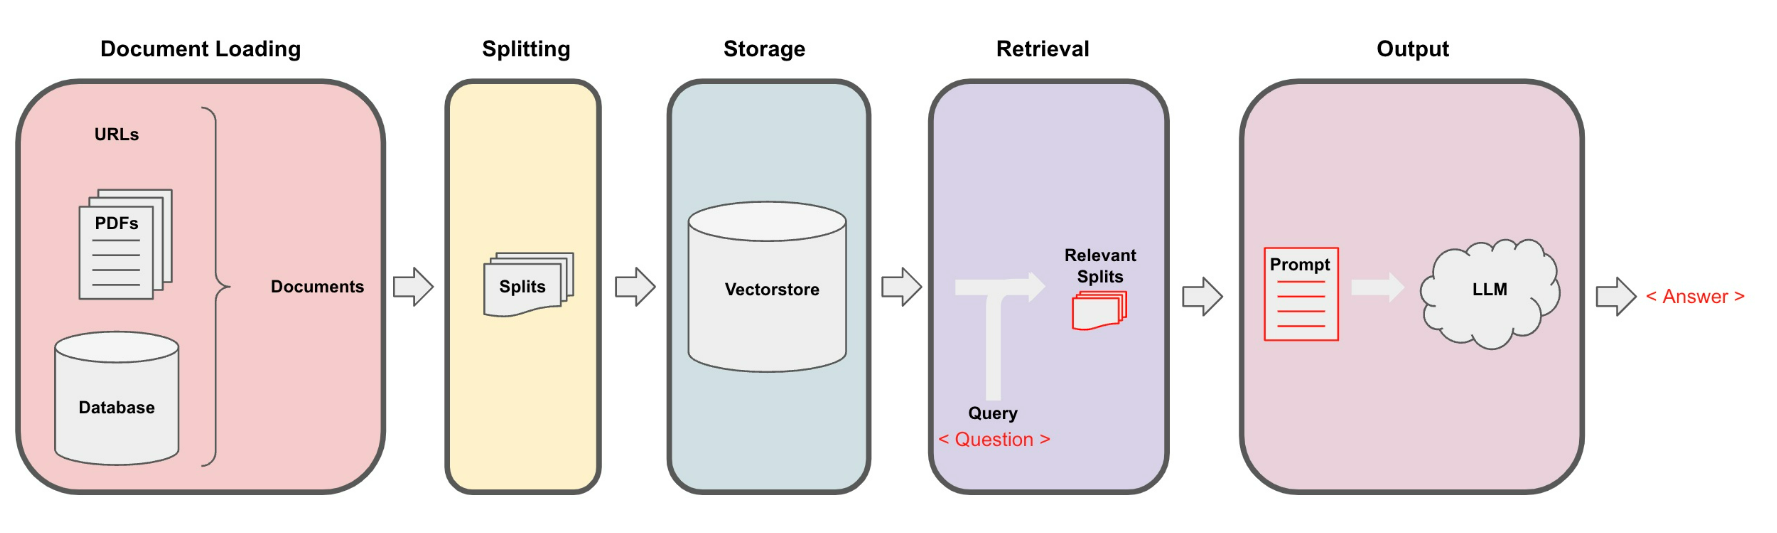
\includegraphics[width=1\textwidth]{Images/Pipeline.png}
    \caption{Overview of the Process for Chatting with Data}
    \label{fig:CHTBT}
\end{figure}

\end{document}
